The following activity diagrams show the basic flow of activities in the toll system. A customer can check in, check out or buy a toll tag. A manager can get a statistical report for a certain time period. The enterprise manager can also change the price of toll tags and tickets.

\begin{figure}[H]
	\centering
	\begin{minipage}{0.3\textwidth}
	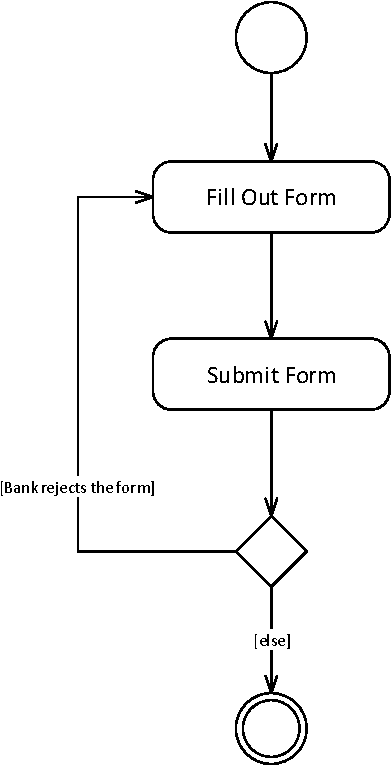
\includegraphics[width=\textwidth]{img/activity_diagram/buy_toll_tag}
	\caption{Activity diagram showing the process of buying a toll tag.}
	\end{minipage}
	\hfill
	\begin{minipage}{0.5\textwidth}
	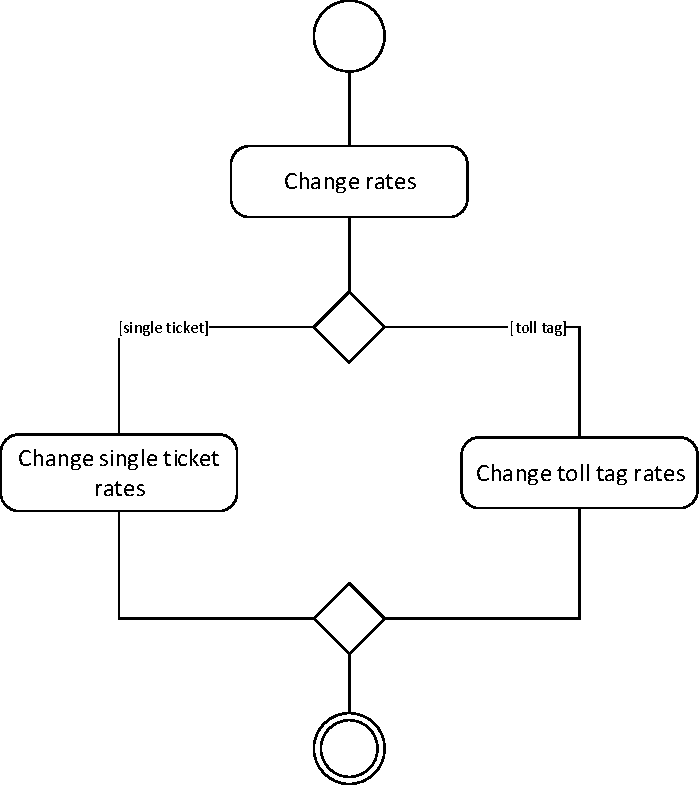
\includegraphics[width=\textwidth]{img/activity_diagram/change_rates}
	\caption{Activity diagram showing the process of changing the rate for toll tags or tickets.}
	\end{minipage}
\end{figure}


\begin{figure}[H]
	\centering
	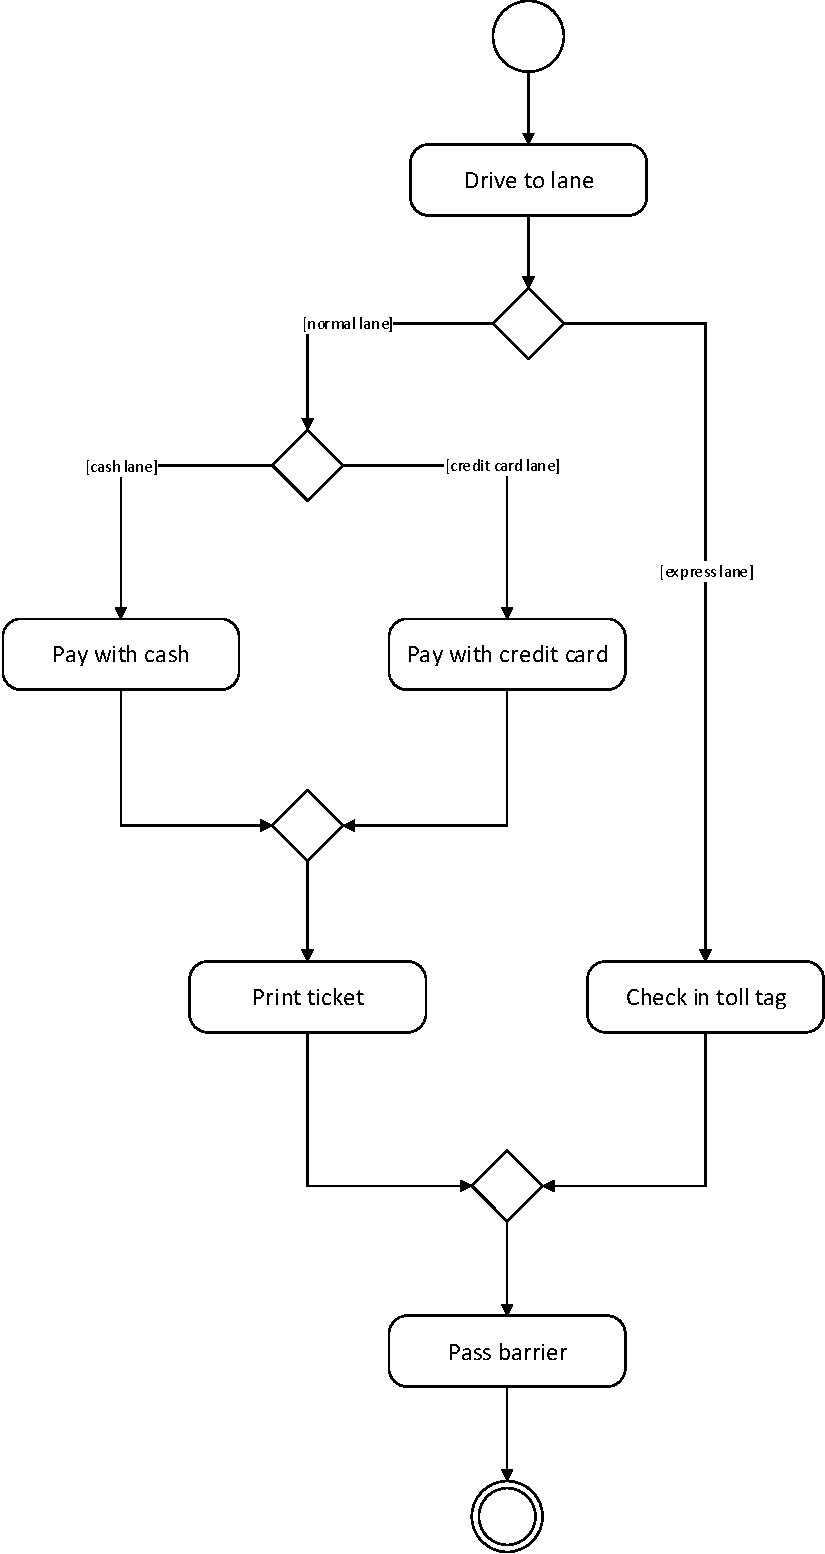
\includegraphics[width=0.3\textwidth]{img/activity_diagram/check_in}
	\caption{Activity diagram showing how a customer checks in.}
\end{figure}

\begin{figure}[H]
	\centering
	\begin{minipage}{0.4\textwidth}
	\centering
	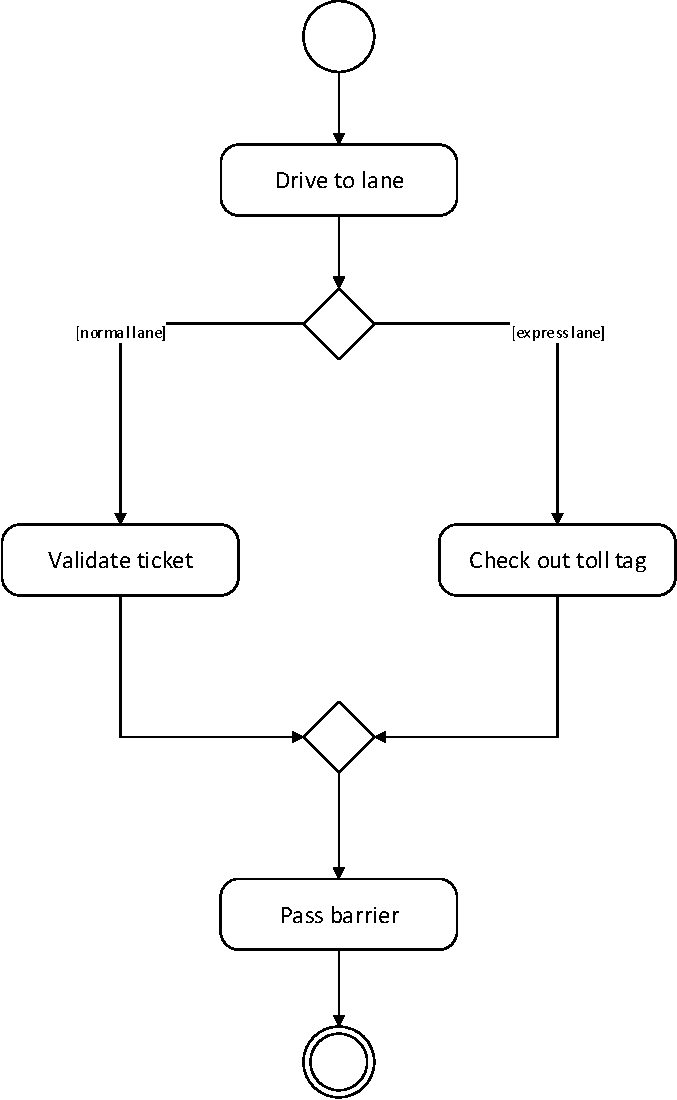
\includegraphics[width=0.7\textwidth]{img/activity_diagram/check_out}
	\caption{Activity diagram showing how a customer checks out.}
	\end{minipage}
	~
	\begin{minipage}{0.3\textwidth}
	\centering
	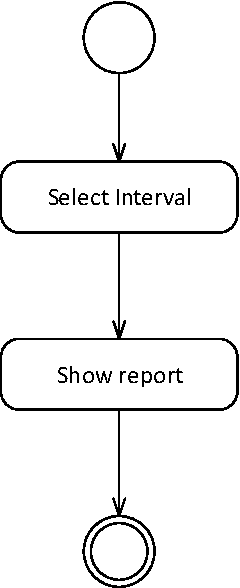
\includegraphics[width=0.4\textwidth]{img/activity_diagram/show_report}
	\caption{Activity diagram showing how a manager gets a report.}
	\end{minipage}
\end{figure}